\documentclass{article}
\usepackage{preamble}
\input{preamble}
\graphicspath{ {images/} }
%%%%%%%%%%%%%%%% Document %%%%%%%%%%%%%%%%
\begin{document}
\begin{center}
{\huge \underline{Variational Methods}}
\end{center}
\tableofcontents
\section*{Math Intro}
\href{https://users.utcluj.ro/~rdanescu/PI-L10e.pdf}{Noise Modeling}

\subsection*{Noise Modelling}
We write $f(i,j) = s(i,j)+n(i,j)$, where $s$ is true signal, $n$ is noise, and $f$ is the acquired signal (noisy). 

Noise can be modeled by a histogram or a PDF which is superimposed on the PDF of the original image $s$. 
\begin{definition}[Salt And Pepper Noise]  $n$ takes only two values - $0$ (black, pepper) or $255$ (white, salt). 
\begin{figure}[H] \centering 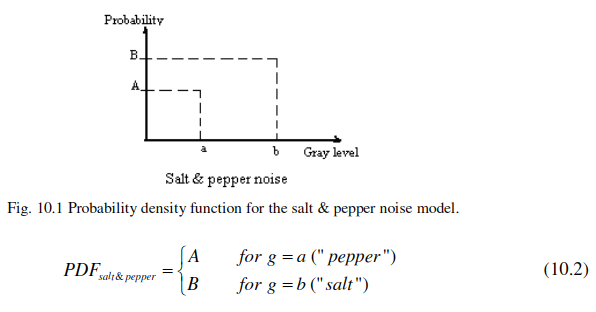
\includegraphics[height=0.2\textheight,width=0.9\textwidth,keepaspectratio]{saltAndPepperNoise}  \label{fig:saltAndPepperNoise} \end{figure}
\end{definition}

\begin{definition}[Gaussian Noise] 
\begin{figure}[H] \centering 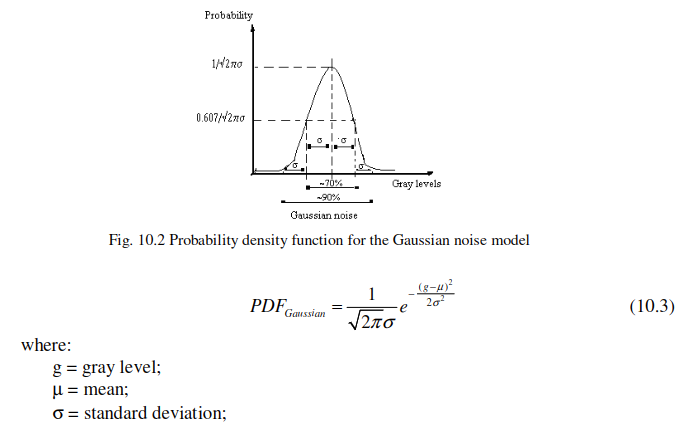
\includegraphics[height=0.3\textheight,width=0.9\textwidth,keepaspectratio]{gaussianNoise} \caption{Gaussian noise} \label{fig:gaussianNoise} \end{figure}
\end{definition}

\begin{definition}[White Noise]  A random vector is said to be a white noise vector if its components each have a PDF with zero mean and finite variance, \textbf{and are statistically independent}. That is, their joint PDF must be the product of the distributions of the individual components.  

If, in addition to being independent, every variable in the vector $w$ has a normal distribution with zero mean  and the same variance $\sigma ^2$, this vector is said to be a Gaussian white noise vector. The joint distribution of $w$ is the multivariate normal distribution.  
\end{definition}



\section{Week 1}
\subsection{Energy and Optimization}
\begin{definition}[Acquisition Model] 
\begin{equation*}
  \boxed{ f = g \ast H + n}
\end{equation*}
  where $f$ is observed image (signal), $g$ is clean image, $n$ is AWGN, and $H$ is known/estimated blur kernel. 

  \begin{figure}[H] \centering 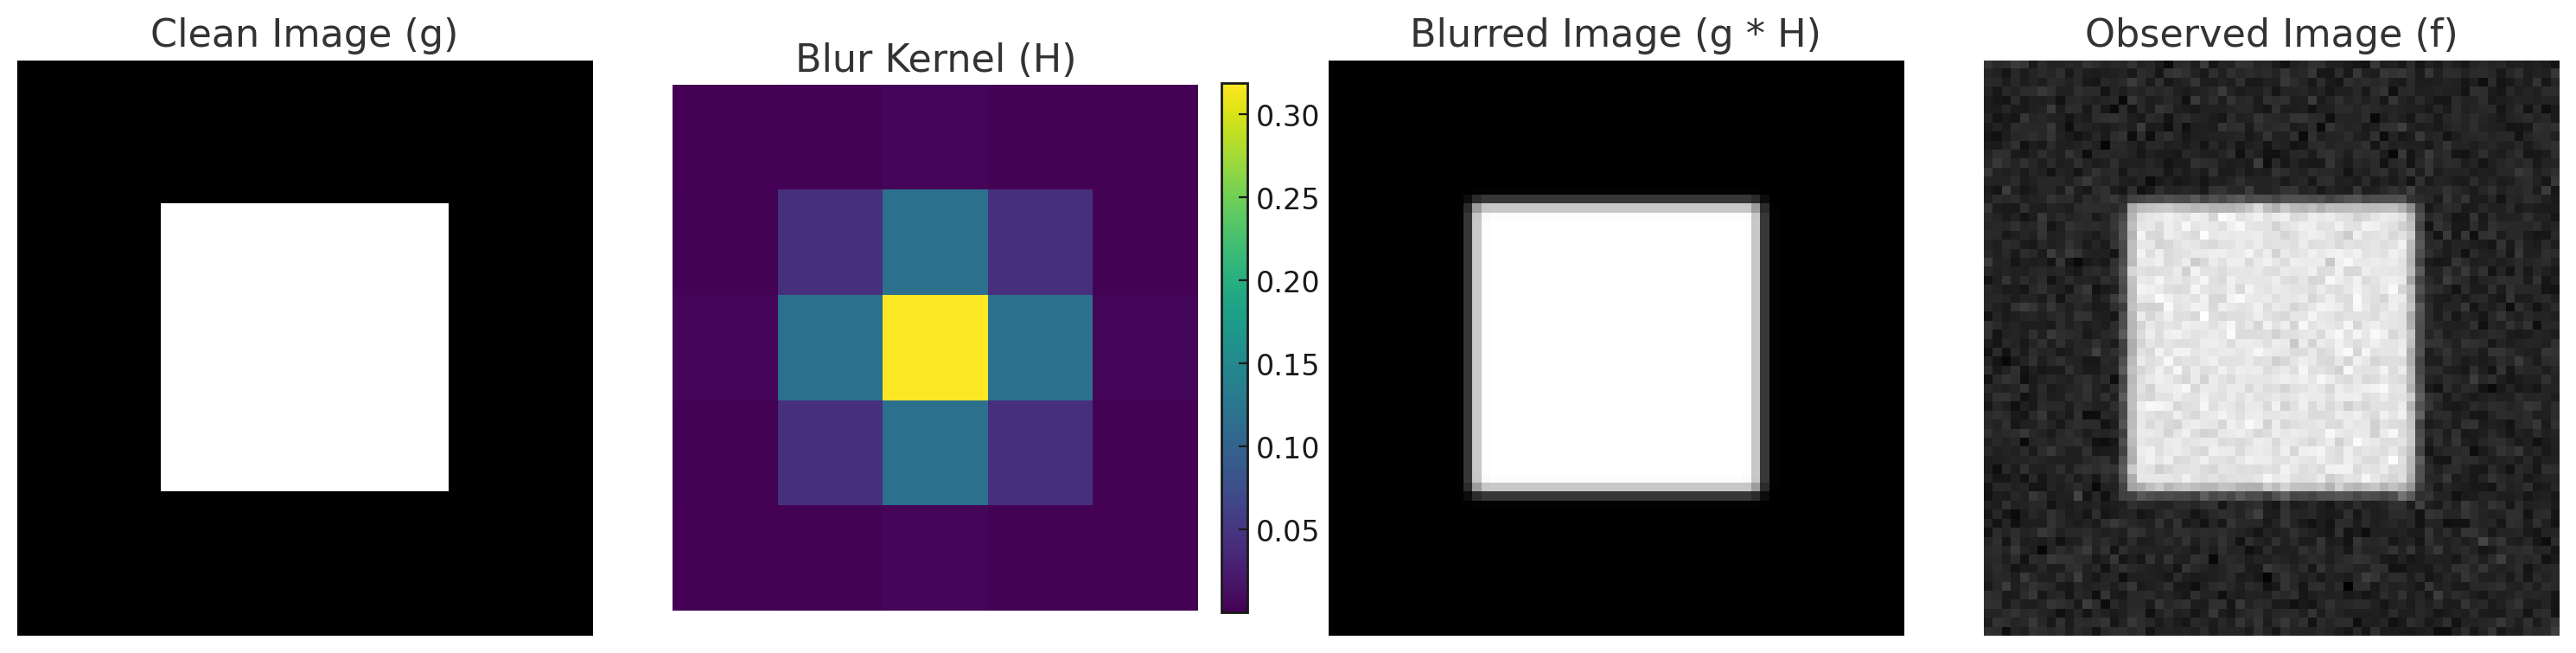
\includegraphics[width=0.9\textwidth,keepaspectratio]{acquisitionProcess.png} \caption{Acquisition Process} \label{fig:acquisitionProcess.png} \end{figure}
\end{definition}

\begin{definition}[Total Variation Energy] 
  Given a signal $u$, we define its total variation by:
\[
  J_{TV}(u) \stackrel{\text{ def }}{=}  \int_{\Omega} | \bm{\nabla}  u(x) | \d{x}
\]
\end{definition}

\begin{definition}[Fidelity Energy] 
  For two signals $u,v$ Fidelity measures how similar are they. For example, we can use the $L2$ norm:
  \[
    E_{\text{Fidelity}} = \lVert u - v \rVert ^2_2
  \]
  
\end{definition}
\begin{example}[Optimization Formulation of the Acquisition Process]
  Let $f = g \ast H + n$ as defined above. We can define the problem of finding $g$ as :
  \[
    \text{Solution } u, \quad   u = \argmin_{u} E_{\text{smoothness}}(u) + \lambda E_{\text{Fidelity}}(u,f) = J_{TV}(u) + \lVert f- u \ast H \rVert_2 ^2
  \]
\end{example}

\subsection{Calculus of Variations}
In finite-dimensional calculus, the derivative of a function provides a linear approximation that describes how the function changes in response to small changes in its input. When we extend our study to infinite-dimensional spaces, such as function spaces in functional analysis, we need a generalized notion of derivatives to capture how functions behave in these settings. This leads us to the concepts of Gâteaux and Fréchet derivatives, which serve as tools to analyze and approximate functions between infinite-dimensional normed vector spaces (Banach spaces).

What We Expect of Such Derivatives:
\begin{itemize}

  \item  Linearity: The derivative should be a linear operator that approximates the change in the function.
  \item Continuity: For the approximation to be meaningful, especially in the Fréchet sense, the linear operator should be continuous.
  \item  Directional Sensitivity: The Gâteaux derivative captures the rate of change of the function in a specific direction, similar to the directional derivative in finite dimensions.
\item  Uniform Approximation: The Fréchet derivative provides a uniform approximation over all directions, akin to the total derivative.
\end{itemize}



\begin{definition}[Gâteaux Derivative]  Let $X$ be a Banach space, $u,v \in X$, and $E: X \to \mathbb{R}$. The Gâteaux Derivative of $E$ at $u \in X$ is defined as:
\[
  \delta E(u ; v) =   E'(u ; v) \stackrel{\text{ def }}{=}  \lim_{\lambda \to 0^{+}} \frac{E(u + \lambda v) -E(u)}{\lambda} = \frac{d E(u + \lambda v)}{d \lambda} \Big|_{\lambda=0} 
\]
We call $v$ a \textbf{variation}, we call \textit{$\lambda v$} a \textbf{perturbation}. 
We  assume zero contribution on the boundary, i.e. $v|_{\Omega} = 0$. 
We also assume that $E$ is Gâteaux differentiable, that is, for all $v$ we reach the same limit.  
We call $\delta E(u ; v)$ the \textbf{first variation} or \textbf{Gâteaux variation} of $E$ at $u \in X$. 

The existence of such the Gâteaux derivative presupposes that:
\begin{itemize}
  \item $E(u)$ is defined 
  \item $E(u + \lambda v)$ is defined for all sufficiently small $\lambda$. 
\end{itemize}
\end{definition}

\begin{remark} In the expression $\frac{d E(u + \lambda v)}{d \lambda}$, we are really looking at the function $\lambda \to E(u+ \lambda v)$, and differentiating it with respect to $\lambda$. The expression $\frac{d E(u+\lambda v)}{d \lambda} \Big|_{\lambda = 0}$ assumes that $\frac{d E(u + \lambda v)}{d \lambda}$ is defined at $\lambda = 0$. 

\end{remark}

\begin{theorem}[Uniqueness of the Gâteaux Derivative]
\end{theorem}

\begin{definition}[Gâteaux Differentiable]  We say a function $E: X \to Y$ is Gâteaux differentiable at $u \in X$, if there is a bounded and linear operator $D_{E}(u) : X \to Y$ such that :
\[
  \lim_{\lambda \to 0} \frac{ E(u+ \lambda v) - E(u) }{\lambda} = D_{E}(u)(v)
\]
for every $v \in X$. We call the operator $D_{E}(u)$ the \textbf{Gâteaux derivative} of $E$ at $u$. It gives the instantaneous rate of change $E$ at $u$ in the direction of $v$. 
\end{definition}


\begin{example} Let $X$ be $C^{1}[a,b]$, and let $E: C^{1}[a,b] \to \mathbb{R}$ be  $E(u) = \int_{a}^{b} |u(t)| ^2 \d{t}$. Then, for each $u \in C^{1}[a,b]$ we have that the integral is finite, and hence $E$ is defined. Let $v \in C^{1}[a,b]$ be an arbitrary direction. Then:
\begin{align*}
 \frac{E(u+\lambda v)-E(v)}{\lambda} &= \frac{1}{\lambda} \int_{a}^{b}  (u(x) +\lambda v(x) ) ^2 - u(x) ^2 \d{x}  = 2 \int_{a}^{b} u(x) v(x) \d{x} + \lambda \int_{a}^{b} (v(x)) ^2 \d{x} 
\end{align*}
Letting $\lambda \to 0$,  we get:
\[
  \frac{d E(u+\lambda v)}{d \lambda} \Big|_{\lambda = 0} = \delta E(u ; v) =  2 \int_{a}^{b} \big( u(x) v(v) \big) \d{x}
\]
  or equivalently, define $f(\lambda) = E(u + \lambda v) = \int_{a}^{b} | (u + \lambda v)(x) |  \d{x}$. Then $f'(\lambda) = 2 \int_{a}^{b} (u v)(x) \d{x} + \lambda \int_{a}^{b} v(x) ^2 \d{x}$, and $\delta E(u ; v) = f'( \lambda) \Big|_{\lambda = 0} = f'(0) = 2 \int_{a}^{b} (uv) (x) \d{x}$ .

Since this exists for all $v \in C^{1}[a,b]$, we say that $E$ is Gâteaux differentiable at $u \in C^{1}[a,b]$, and we have its \textit{Gâteaux derivative}:
\[
  D_{E}(u) (v) = 2 \int_{a}^{b} \big( u(x) v(x)  \big) \d{x}
\]
\end{example}


\begin{example}[Non Gâteaux differentiable] Let $E: C^{1}[0,1] \to \mathbb{R}$ be the functional defined, at $u \in C^{1}[0,1]$ by:
\[
  E(u) := \int_{0}^{1} |u(x)| \d{x}
\]
  Then, at "point" $u(x) := 0$, and for direction $v(x) := x$, we have :
\[
  E(u+\lambda v) = \int_{0}^{1} |u(x) + \lambda v(x)| \d{x} = \int_{0}^{1} |0 + \lambda x| \d{x} = | \lambda | \int_{0}^{1} |x| \d{x} = \frac{ | \lambda| }{2}
\]
And:
\[
  E(u+\lambda v) - E(u) = \frac{ | \lambda| }{2}
\]
i.e.:
\[
  \frac{E (u + \lambda v) - E(v) }{\lambda} =   \frac{1}{\lambda} \frac{| \lambda |}{2} = \begin{cases} 1/2, & \lambda > 0 \\ -1/2, & \lambda < 0 \\ \text{undefined}, & \lambda = 0 \end{cases} 
\]
Therefore:
$\delta E(u ; v)$ does not exist, since 
 \[
   \lim_{\lambda \to 0} \frac{E(u + \lambda v)-E(u)}{ \lambda} 
 \]
  does not exist, particularly because it has different values when   approaching from different sides. 

Equivalently, we can define
\[
  f (\lambda) = E(u + \lambda v) = \int_{0}^{1} | u + \lambda v |(x)  \d{x} = | \lambda |
  \int_{0}^{1} | x | \d{x} = | \lambda | \frac{1}{2}. 
\] 
Differentiating with respect to $\lambda$, we get:

\[
  f'(\lambda) =  \begin{cases} 1/2, & \lambda >0 \\ -1/2,  & \lambda < 0 \\ \text{undefined}, & \lambda = 0  \end{cases} 
\]
  Therefore we have that $\delta E (u ; v) = f'(0)$ is undefined. 
\end{example}



\begin{definition}[Fréchet Derivative] Let $X,Y$ be normed vector spaces, and $f: X \to Y$.   The Fréchet derivative of $f$ at a point $x \in X$ is a bounded linear operator $A: X \to Y$ such that:

\[
  \lim_{\lVert h \rVert \to 0} \frac{ \lVert f(x+h) - f(x) - Ah \rVert_Y  }{ \lVert h \rVert_X  } = 0
\]
 \end{definition}

\section{Perona-Malik}
\begin{theorem}[Finite Difference and Flow] \label{th:FDAndFlow} Let $u$ be a 1D array. 
\begin{itemize}
\item \ul{Forward-Difference at $i$ measures \textbf{inflow} from right}: Define forward difference at $i$ by:
\[ u[i+1]-u[i]  \]
When $u[i+1] > u[i]$ there will be flow from $i+1$ into $i$. Therefore the FD at $i$ measures the (signed) inflow from $i+1$ to $i$. 

\item \ul{Negative Forward-Difference at $i$ measures \textbf{outflow} from $i$ to right} The expression:
\[
    u[i]-u[i+1]
\]
  when $u[i] > u[i+1]$, there will be flow from $i$ to $i+1$, hence this measures \textbf{outflow} from $i$ to $i+1$. 

Specifically, when at $i-1$, the expression:
\[
 u[i-1]-u[i]
\]
 measures \textbf{outflow} from $(i-1)$ to $i$, which is \textbf{inflow} into $i$ from $i-1$.
  \end{itemize}
\end{theorem}
\begin{theorem}[Perona-Malik]
Fick's Law tells us that 
\begin{equation}
  \bm{J} = - c \bm{\nabla} u
\end{equation}
Also the continuity equation is:
\begin{equation}
  \frac{\partial u}{\partial t} = - \operatorname{div} \bm{J}
\end{equation}
Hence $\bm{J}$ measures the flux, i.e. the net \textbf{outflow} from an infinitesimal volume, like the outflow from pixel (i,j)

Combining Fick's Law with the continuity equation, we get the Perona-Malik equation:
\[
  \frac{\partial u}{\partial t}  = \operatorname{div}(c \bm{\nabla}  u)
\]
  I.e. the amount of change of $u$ is equal to $\operatorname{div}(c \bm{\nabla} u)$. Hence $\operatorname{div}(c \bm{\nabla} u)_{i,j}$ measures the net \textbf{inflow} into $(i,j)$ pixel. 

Focusing on the $x$-axis, we wish to measure the net \textbf{inflow} into $(i,j)$ pixel along the $x$-axis, which is $\operatorname{div}_{x}(c \bm{\nabla} u)_{i,j}$

At $(i,j)$ we have:
\[
\begin{alignedat}{3}
  \operatorname{div}_{x}(c \bm{\nabla} u)_{i,j} = \text{net inflow into $(i,j)$} 
    &= \Big( \text{inflow into $(i,j)$ from $(i, j+1)$} \Big) 
    &&+ \Big( \text{inflow into $(i,j)$ from $(i, j-1)$} \Big) \\
  &\approx \Big( u[i,j+1] - u[i,j] \Big) 
    &&+ \Big( u[i,j-1] - u[i,j] \Big)
\end{alignedat}
\]

\end{theorem}





\end{document}

